
\documentclass[a4paper,12pt]{article}
%%%%%%%%%%%%%%%%%%%%%%%%%%%%%%%%%%%%%%%%%%%%%%%%%%%%%%%%%%%%%%%%%%%%%%%%%%%%%%%%%%%%%%%%%%%%%%%%%%%%%%%%%%%%%%%%%%%%%%%%%%%%%%%%%%%%%%%%%%%%%%%%%%%%%%%%%%%%%%%%%%%%%%%%%%%%%%%%%%%%%%%%%%%%%%%%%%%%%%%%%%%%%%%%%%%%%%%%%%%%%%%%%%%%%%%%%%%%%%%%%%%%%%%%%%%%
\usepackage{graphicx,hyperref,mathpple,amsmath,exscale,setspace,xcolor}
\usepackage[left=20mm,right=20mm,top=20mm,bottom=20mm]{geometry}
\usepackage{pdflscape,showkeys,changepage}
\usepackage[round]{natbib}

\setcounter{MaxMatrixCols}{10}
%TCIDATA{OutputFilter=LATEX.DLL}
%TCIDATA{Version=5.50.0.2953}
%TCIDATA{<META NAME="SaveForMode" CONTENT="2">}
%TCIDATA{BibliographyScheme=BibTeX}
%TCIDATA{Created=Wednesday, May 03, 2023 13:45:06}
%TCIDATA{LastRevised=Wednesday, November 22, 2023 12:55:15}
%TCIDATA{<META NAME="GraphicsSave" CONTENT="32">}
%TCIDATA{<META NAME="DocumentShell" CONTENT="Standard LaTeX\Blank - Standard LaTeX Article">}
%TCIDATA{CSTFile=40 LaTeX article.cst}

\let\oldref\ref
\AtBeginDocument{
\let\oldref\ref\renewcommand{\ref}[1]{(\oldref{#1})}
\newcommand{\bsq}{\begin{subequations}}\newcommand{\esq}{\end{subequations}}
\newcommand{\bls}{\begin{landscape}}\newcommand{\els}{\end{landscape}}
\renewcommand\showkeyslabelformat[1]{{\parbox[t]{\marginparwidth}{\raggedright\footnotesize\url{#1}}}}
\newcommand{\intxt}[1]{\intertext{#1}}\newcommand{\BAW}[1]{\begin{adjustwidth}{-#1mm}{-5mm}}\newcommand{\EAW}{\end{adjustwidth}}
\newcommand{\vsp}[1]{\vspace*{#1mm}}\newcommand{\hsp}[1]{\hspace*{#1mm}}  }
\renewcommand\section{\@startsection{section}{1}{\z@}{-2.5ex \@plus -1ex \@minus -.2ex}{0.01ex \@plus.2ex}{\Large\bfseries}}
\renewcommand\subsection{\@startsection{subsection}{1}{\z@}{-1.5ex \@plus -1ex \@minus -.2ex}{0.01ex \@plus.2ex}{\large\bfseries}}
\makeatletter
\renewcommand*{\@fnsymbol}[1]{\ensuremath{\ifcase#1\or *\or
    \#\or \star\or \bowtie\or \star\star\or \ddagger\ddagger \else\@ctrerr\fi}}
\makeatother
\allowdisplaybreaks
\IfFileExists{C:/swp55/TCITeX/TeX/LaTeX/SWmacros/tcilatex.tex}{\input{tcilatex}}{}
\graphicspath{{../graphics/}{graphics/}}
\definecolor{myred}{rgb}{.50,.10,.10}
\definecolor{mygrn}{rgb}{.10,.35,.10}
\definecolor{myblu}{rgb}{.10,.10,.35}
\hypersetup{colorlinks,citecolor=myblu,filecolor=mygrn,linkcolor=myred,urlcolor=mygrn,breaklinks=true}
\setstretch{1.2345}
\setlength{\parskip}{7pt}

\begin{document}


\section{Clark87}

The UC\ model of Clark (1987) is a generalisation of the HP--Filter (a local
linear trend model) that can be expressed as an SSM taking the following
form:\bsq\label{clark0}%
\begin{align}
y_{t}& =y_{t}^{\ast }+\tilde{y}_{t} \\
\Delta y_{t}^{\ast }& =g_{t-1}+\sigma _{1}\varepsilon _{1t} \\
\Delta g_{t}& =\sigma _{2}\varepsilon _{2t} \\
a(L)\tilde{y}_{t}& =\sigma _{3}\varepsilon _{3t},
\end{align}%
\esq where the shocks $\left\{ \varepsilon _{it}\right\} _{i=1}^{3}$ are
assumed to be $i.i.d.$ standard normal and mutually uncorrelated, with
standard deviation $\sigma _{i}$ and $a(L)$ is commonly assumed to be a
stable AR(2), so that $a(L)=(1-a_{1}L-a_{2}L^{2})$. The only observable is $%
y_{t}$ (generally 100 times) the log of real GDP and with the cycle (denoted
by $\tilde{y}_{t}$) now allowed to be serially correlated, following a
stationary AR(2) process. There are 3 shocks in the model.

The `\emph{numbered}' shock to `\emph{named}' shock mapping is:%
\begin{equation}
\begin{bmatrix}
\varepsilon _{1t} \\
\varepsilon _{2t} \\
\varepsilon _{3t}%
\end{bmatrix}%
=%
\begin{bmatrix}
\varepsilon _{t}^{y^{\ast }} \\
\varepsilon _{t}^{g} \\
\varepsilon _{t}^{\tilde{y}}%
\end{bmatrix}%
.
\end{equation}

The (standard)\ SSM\ for ML\ estimation is:%
\begin{align}
y_{t}& =%
\begin{bmatrix}
1 & 0 & 1 & 0%
\end{bmatrix}%
\begin{bmatrix}
y_{t}^{\ast } \\
g_{t} \\
\tilde{y}_{t} \\
\tilde{y}_{t-1}%
\end{bmatrix}%
+0\varepsilon _{t} \\[4mm]
\begin{bmatrix}
y_{t}^{\ast } \\
g_{t} \\
\tilde{y}_{t} \\
\tilde{y}_{t-1}%
\end{bmatrix}%
& =%
\begin{bmatrix}
1 & 1 & 0 & 0 \\
0 & 1 & 0 & 0 \\
0 & 0 & a_{1} & a_{2} \\
0 & 0 & 1 & 0%
\end{bmatrix}%
\begin{bmatrix}
y_{t-1}^{\ast } \\
g_{t-1} \\
\tilde{y}_{t-1} \\
\tilde{y}_{t-2}%
\end{bmatrix}%
+%
\begin{bmatrix}
\sigma _{1} & 0 & 0 \\
0 & \sigma _{2} & 0 \\
0 & 0 & \sigma _{3} \\
0 & 0 & 0%
\end{bmatrix}%
\begin{bmatrix}
\varepsilon _{1t} \\
\varepsilon _{2t} \\
\varepsilon _{3t}%
\end{bmatrix}%
.
\end{align}

\bigskip

The code estimates Clark's 87 model on US GDP\ data from $1947$:Q1 to $2019$%
:Q4. A plot of the smoothed and filtered estimates is shown below.

\begin{figure}[p!]
\centering
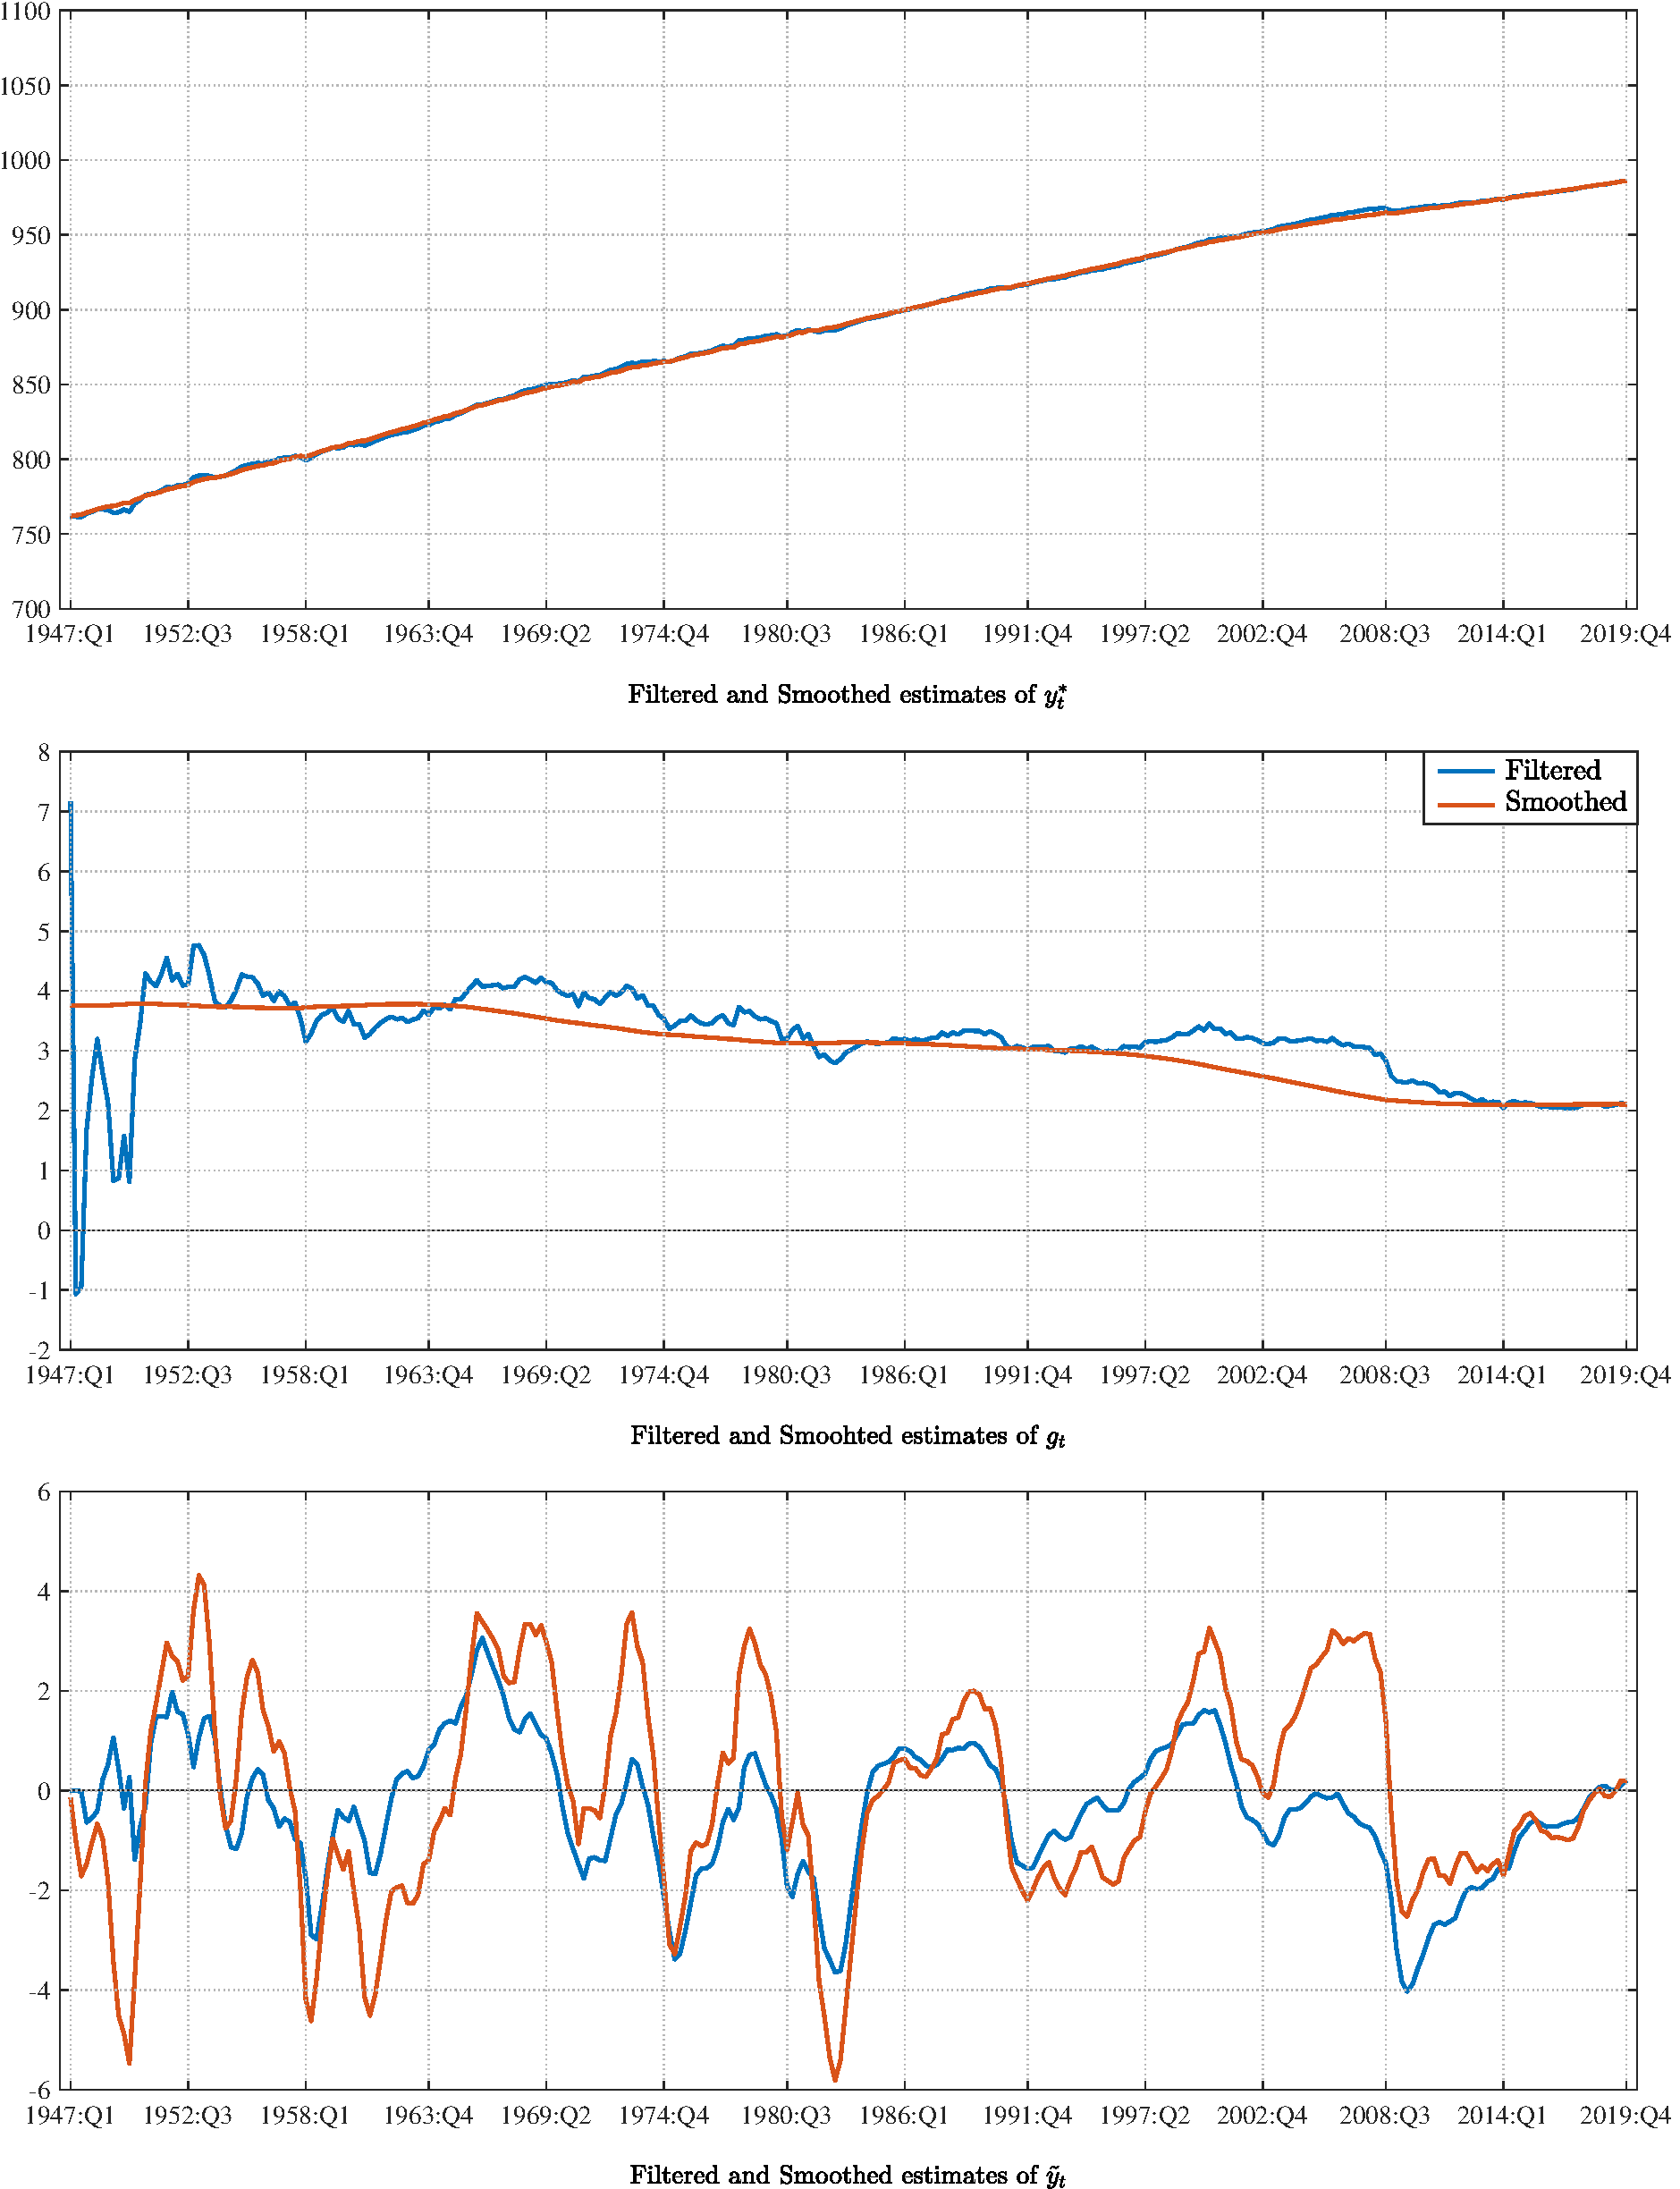
\includegraphics[angle=00, width=1\textwidth,trim={0 0 0 0},clip]{Clark_SSM}
\label{fig:KFS}
\end{figure}

\section{Shock recovery SSM}

\subsection{SSM with lagged states}

Kurz's (2018) SSM has the following general from:\bsq\label{SSM}%
\begin{align}
\mathsf{Measurement}& :\quad Z_{t}=D_{1}X_{t}+D_{2}X_{t-1}+R\varepsilon _{t}
\label{ssm1} \\
\mathsf{State}& :\quad X_{t}=AX_{t-1}+C\varepsilon _{t},  \label{ssm2}
\end{align}%
\esq where $\varepsilon _{t}\sim MN(0,I_{m})$, $D_{1},D_{2},A,R$ are $C$ are
conformable system matrices, $Z_{t}$ the observed variable and $X_{t}$ the
latent state variable.

\subsection{Clark87 SSM\ for shock recovery}

To assess recovery, re-write the model in \ref{clark0} in `\emph{shock
recovery}' State Space Form (SSF). That is, collect all observables in $%
Z_{t} $ and all shocks (and other state variables)\ in $X_{t}$ to yield:%
\begin{align}
\Delta ^{2}y_{t}& =\Delta ^{2}y_{t}^{\ast }+\Delta ^{2}\tilde{y}_{t}
\label{2diff} \\
& =\sigma _{1}\Delta \varepsilon _{1t}+\Delta g_{t-1}+\Delta ^{2}\tilde{y}%
_{t}  \notag \\
& =\sigma _{1}\Delta \varepsilon _{1t}+\sigma _{2}\varepsilon
_{2t-1}+a(L)^{-1}\sigma _{3}\Delta ^{2}\varepsilon _{3t}  \label{e2lag} \\
\Leftrightarrow a(L)\Delta ^{2}y_{t}& =\sigma _{1}a(L)\Delta \varepsilon
_{1t}+\sigma _{2}a(L)\varepsilon _{2t-1}+\sigma _{3}\Delta ^{2}\varepsilon
_{3t}  \notag
\end{align}%
where $Z_{t}=a(L)\Delta ^{2}y_{t}$ is the only observed variable.

Re-writing these in more convenient form for the SSF yields:%
\begin{align}
\underbrace{a(L)\Delta ^{2}y_{t}}_{Z_{t}}& =a(L)\sigma _{1}\Delta
\varepsilon _{1t}+a(L)\sigma _{2}\varepsilon _{2t-1}+\sigma _{3}\Delta
^{2}\varepsilon _{3t}  \label{eqZ} \\[-5mm]
& =\sigma _{1}\Delta \varepsilon _{1t}-a_{1}\sigma _{1}\Delta \varepsilon
_{1t-1}-a_{2}\sigma _{1}\Delta \varepsilon _{1t-2}  \notag \\
& +\sigma _{2}\varepsilon _{2t-1}-a_{1}\sigma _{2}\varepsilon
_{2t-2}-a_{2}\sigma _{2}\varepsilon _{2t-3}  \notag \\
& +\sigma _{3}\Delta \varepsilon _{3t}-\sigma _{3}\Delta \varepsilon _{3t-1},
\notag
\end{align}%
which can then be written in SSF as:%
\begin{align}
\mathsf{State}:\quad X_{t}& =AX_{t-1}+C\varepsilon _{t} \\
\begin{bmatrix}
\varepsilon _{1t} \\
\varepsilon _{2t} \\
\varepsilon _{3t} \\
\Delta \varepsilon _{1t} \\
\Delta \varepsilon _{1t-1} \\
\varepsilon _{2t-1} \\
\varepsilon _{2t-2} \\
\Delta \varepsilon _{3t}%
\end{bmatrix}%
& =%
\begin{bmatrix}
0 & 0 & 0 & 0 & 0 & 0 & 0 & 0 \\
0 & 0 & 0 & 0 & 0 & 0 & 0 & 0 \\
0 & 0 & 0 & 0 & 0 & 0 & 0 & 0 \\
-1 & 0 & 0 & 0 & 0 & 0 & 0 & 0 \\
0 & 0 & 0 & 1 & 0 & 0 & 0 & 0 \\
0 & 1 & 0 & 0 & 0 & 0 & 0 & 0 \\
0 & 0 & 0 & 0 & 0 & 1 & 0 & 0 \\
0 & 0 & -1 & 0 & 0 & 0 & 0 & 0%
\end{bmatrix}%
\begin{bmatrix}
\varepsilon _{1t-1} \\
\varepsilon _{2t-1} \\
\varepsilon _{3t-1} \\
\Delta \varepsilon _{1t-1} \\
\Delta \varepsilon _{1t-2} \\
\varepsilon _{2t-2} \\
\varepsilon _{2t-3} \\
\Delta \varepsilon _{3t-1}%
\end{bmatrix}%
+%
\begin{bmatrix}
1 & 0 & 0 \\
0 & 1 & 0 \\
0 & 0 & 1 \\
1 & 0 & 0 \\
0 & 0 & 0 \\
0 & 0 & 0 \\
0 & 0 & 0 \\
0 & 0 & 1%
\end{bmatrix}%
\begin{bmatrix}
\varepsilon _{1t} \\
\varepsilon _{2t} \\
\varepsilon _{3t}%
\end{bmatrix}%
.
\end{align}%
\begin{eqnarray*}
\mathsf{Measurement}:\quad Z_{t} &=&D_{1}X_{t}+D_{2}X_{t-1}+R\varepsilon _{t}
\\[-15mm]
Z_{t} &=&%
\begin{bmatrix}
0 & 0 & 0 & \sigma _{1} & -a_{1}\sigma _{1} & 0 & 0 & \sigma _{3}%
\end{bmatrix}%
\begin{bmatrix}
\varepsilon _{1t} \\
\varepsilon _{2t} \\
\varepsilon _{3t} \\
\Delta \varepsilon _{1t} \\
\Delta \varepsilon _{1t-1} \\
\varepsilon _{2t-1} \\
\varepsilon _{2t-2} \\
\Delta \varepsilon _{3t}%
\end{bmatrix}
\\[-15mm]
&&+%
\begin{bmatrix}
0 & \sigma _{2} & 0 & 0 & -a_{2}\sigma _{1} & -a_{1}\sigma _{2} &
-a_{2}\sigma _{2} & -\sigma _{3}%
\end{bmatrix}%
\begin{bmatrix}
\varepsilon _{1t-1} \\
\varepsilon _{2t-1} \\
\varepsilon _{3t-1} \\
\Delta \varepsilon _{1t-1} \\
\Delta \varepsilon _{1t-2} \\
\varepsilon _{2t-2} \\
\varepsilon _{2t-3} \\
\Delta \varepsilon _{3t-1}%
\end{bmatrix}%
+%
\begin{bmatrix}
0 & 0 & 0%
\end{bmatrix}%
\begin{bmatrix}
\varepsilon _{1t} \\
\varepsilon _{2t} \\
\varepsilon _{3t}%
\end{bmatrix}%
\end{eqnarray*}%
$\allowbreak $

Running the shock recovery code\ $\mathtt{Clark87.m}$ we get the following
steady-state diagonal entries:%
\begin{equation*}
\begin{tabular}{ccc}
\hline
Shocks & $P_{t|T}^{\ast }$ & $P_{t|t}^{\ast }$ \\ \hline
$\varepsilon _{1t}$ & $0.5469$ & $0.5989$ \\
$\varepsilon _{2t}$ & $0.9870$ & $1.0000$ \\
$\varepsilon _{3t}$ & $0.4661$ & $0.5153$ \\ \hline
\end{tabular}%
\end{equation*}%
The second shock $\varepsilon _{2t}$ (corresponding to $\varepsilon _{t}^{g}$%
, ie., trend growth) is not recoverable.

Looking at \ref{e2lag}, we see that $\varepsilon _{2t}$ enters with a lag
into the measurement equation. Following the same logic that Adrian used, we
should then get only $\hat{\varepsilon}_{2t-1|t}$ from the Kalman Filter.

Below I plot estimates of the Filtered and Smoothed shocks from the model
fitted to US\ data, where shocks from the SSM in \ref{clark0} are
constructed in line with the equations listed there, ie.,  as $\eta
_{2t|t}=\sigma _{2}\varepsilon _{2t}=\Delta g_{t}$ for the filtered and
smoothed alternatives.

\begin{figure}[p!]
\centering
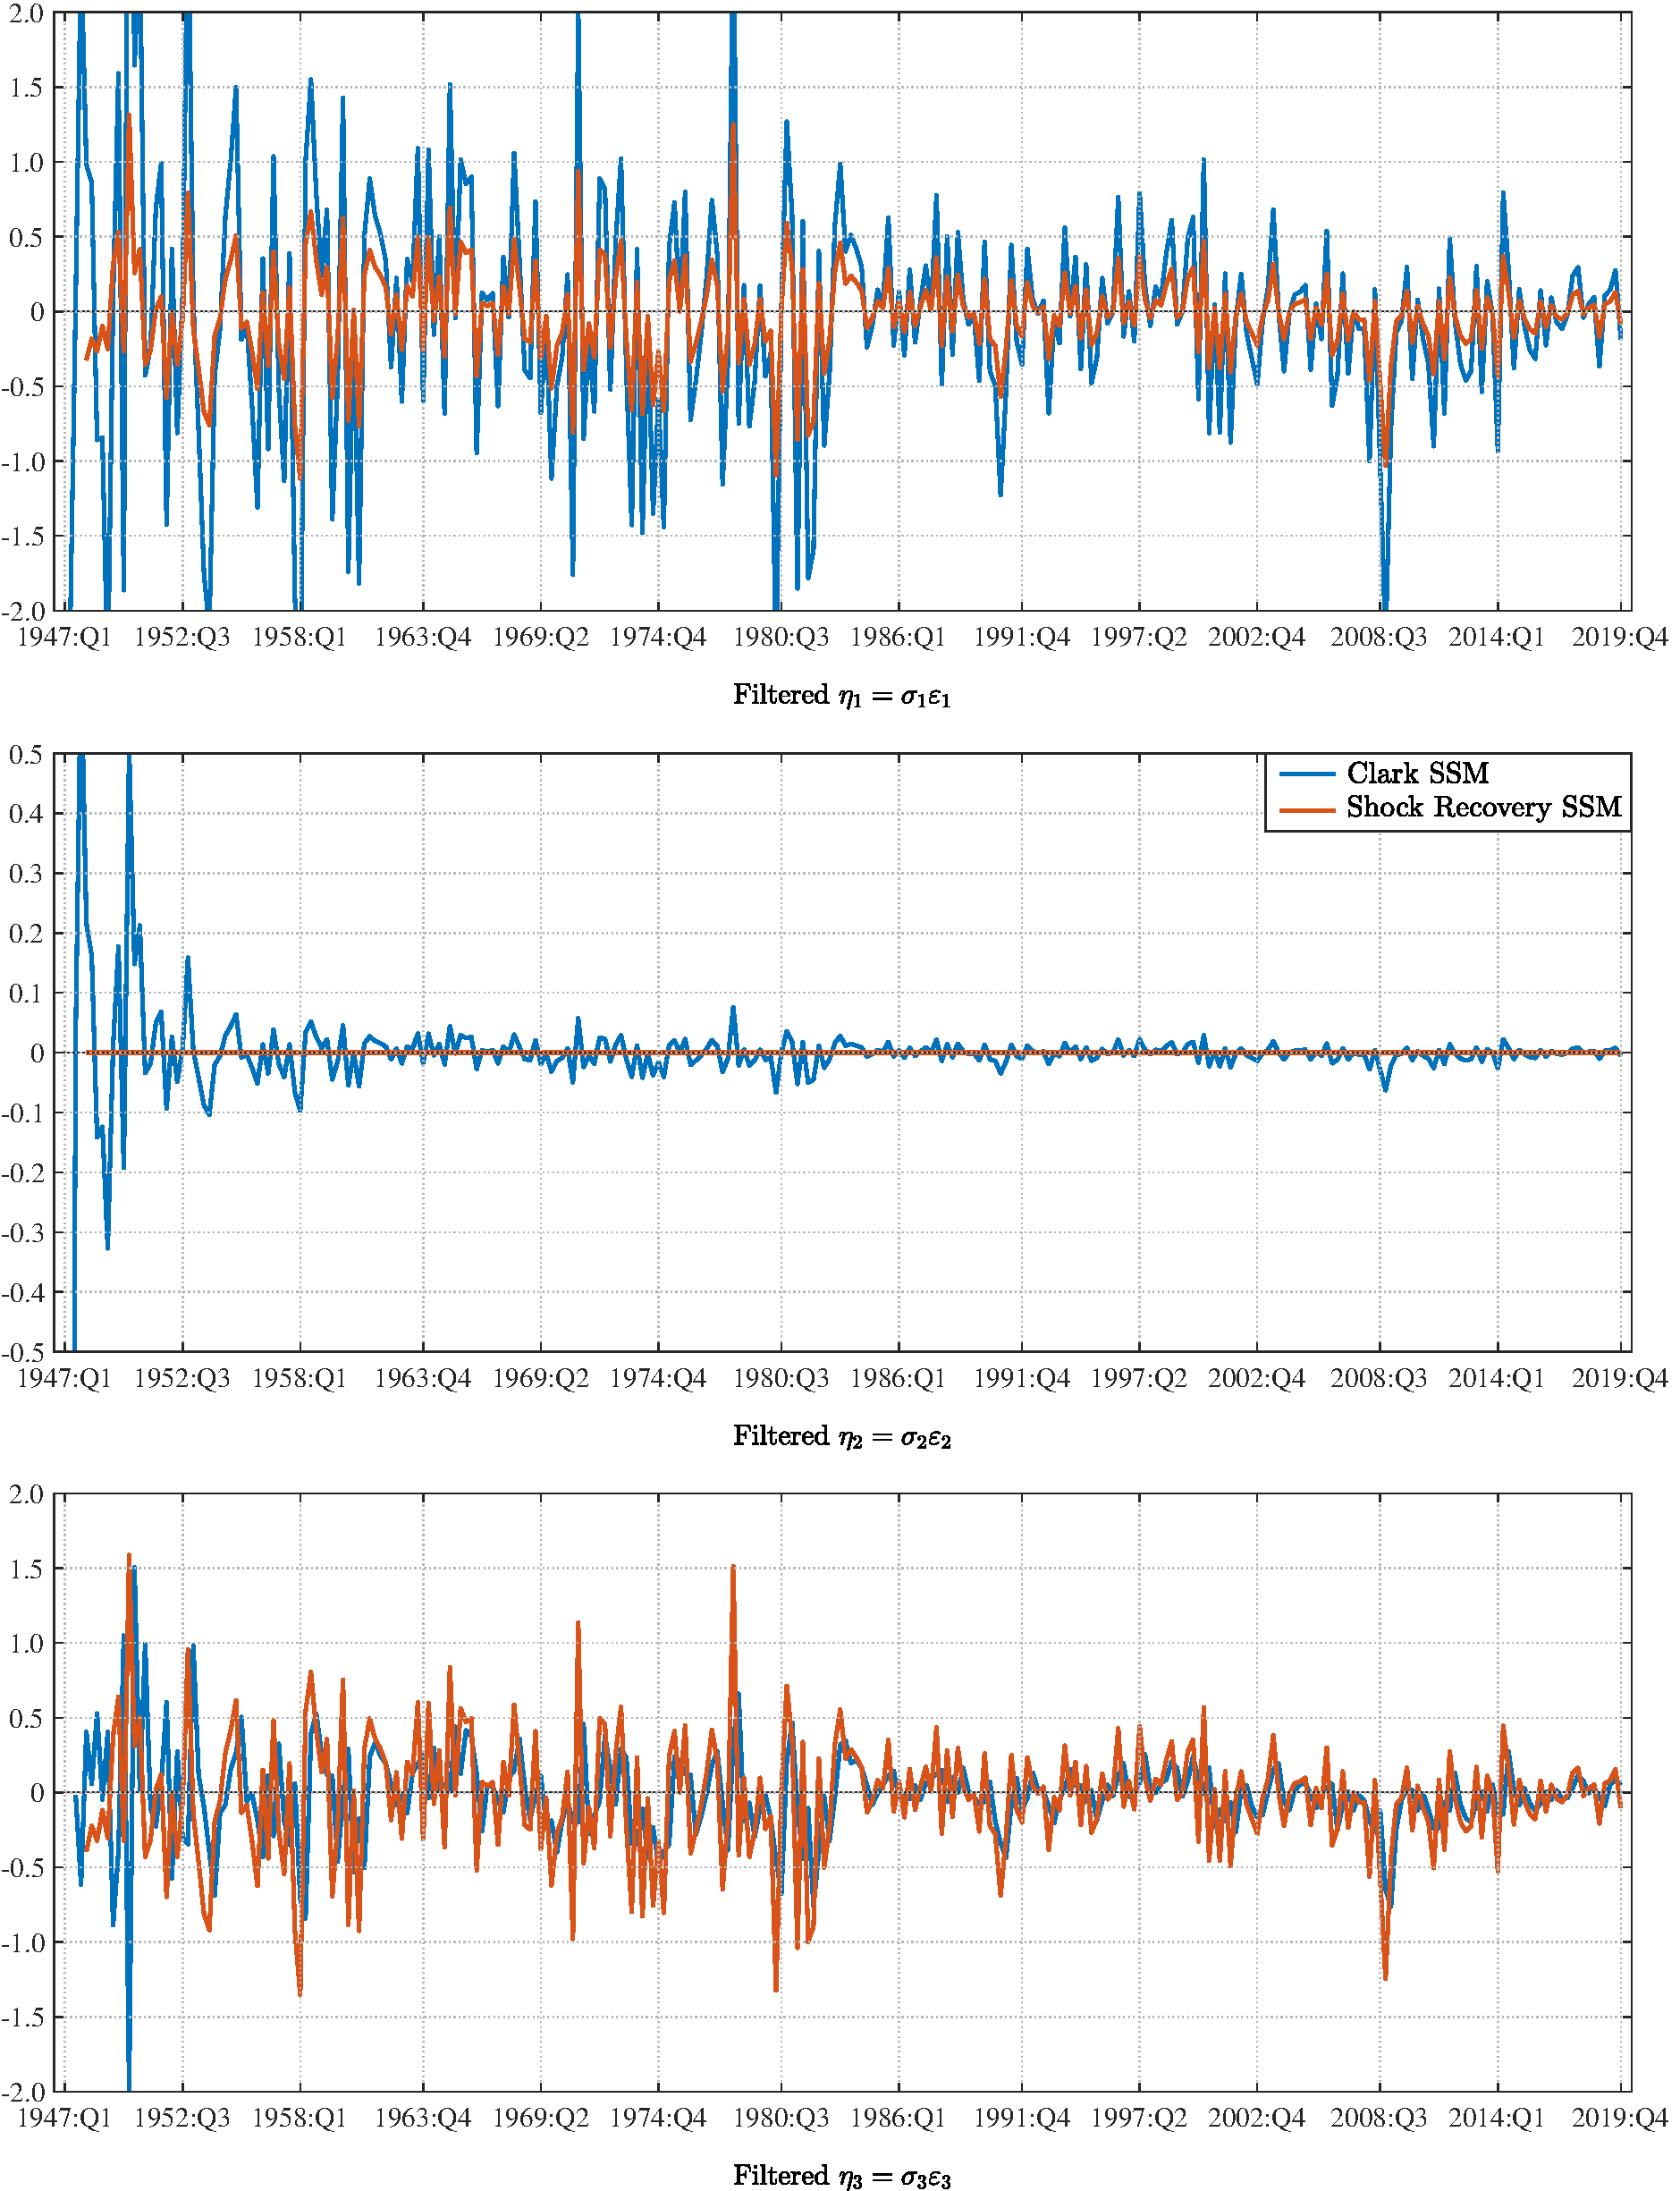
\includegraphics[angle=00, width=1\textwidth,trim={0 0 0 0},clip]{Clark_SSM_Filtered}
\label{fig:KF}
\end{figure}


\begin{figure}[p!]
\centering
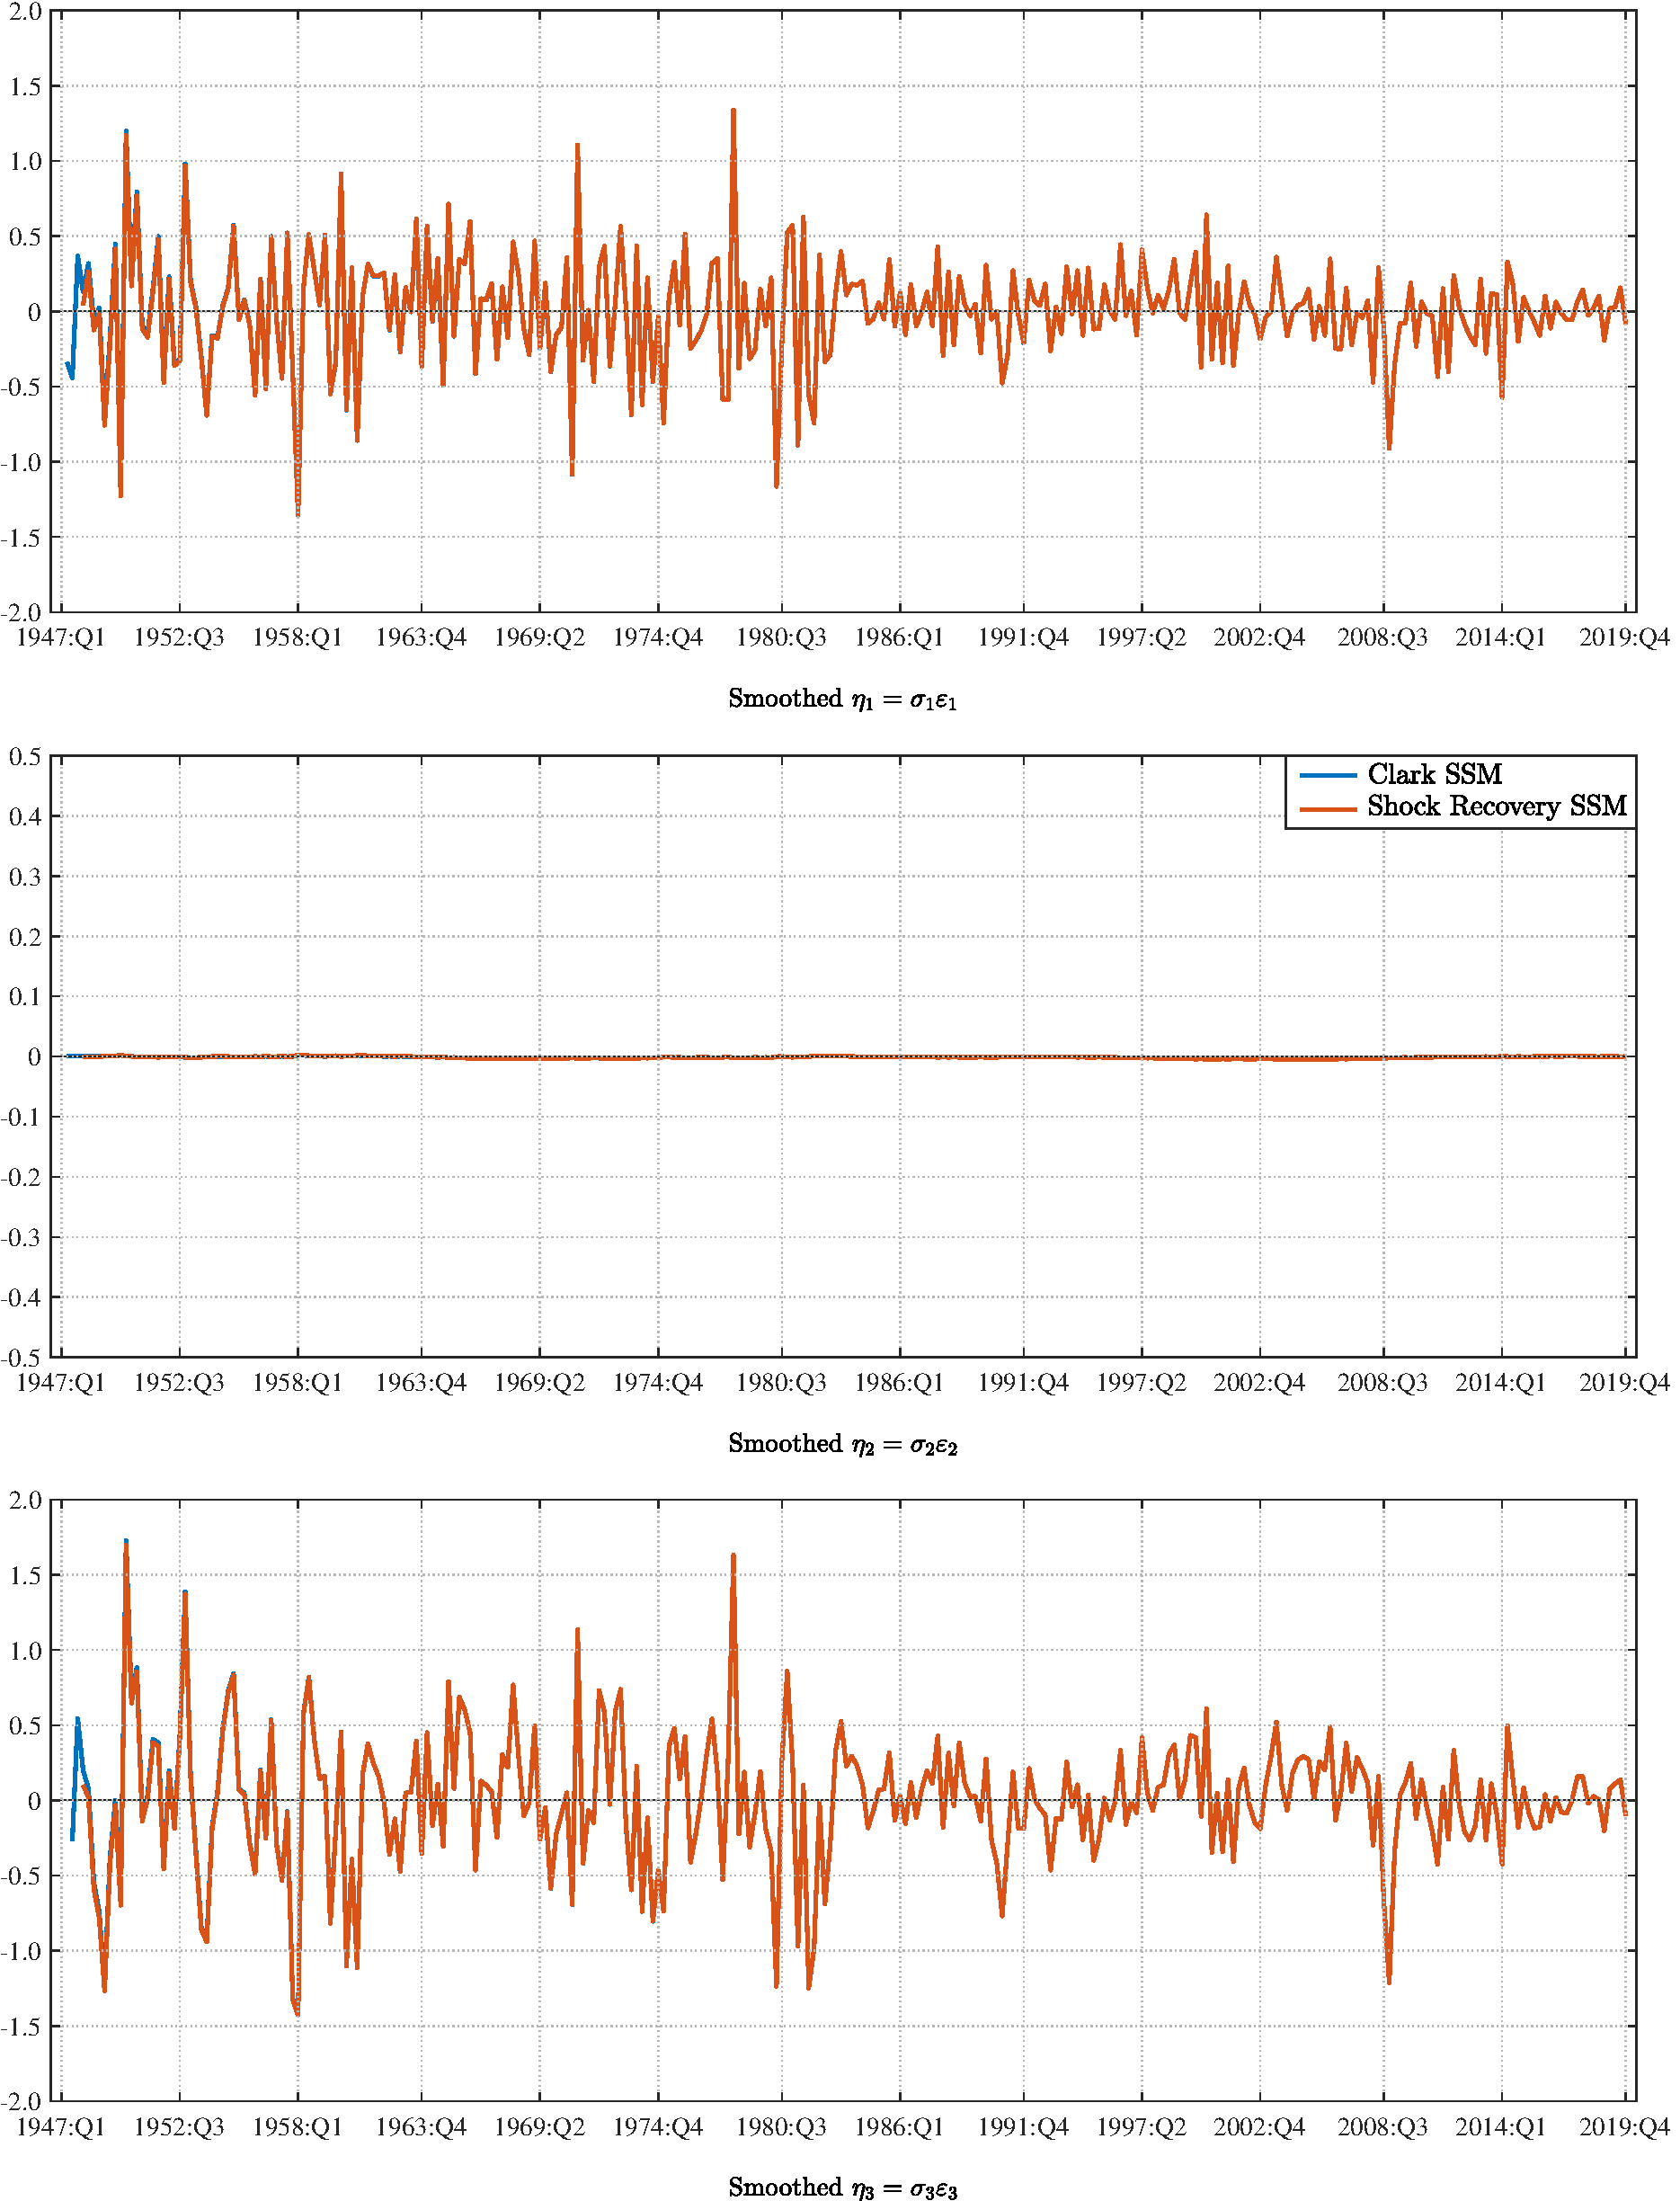
\includegraphics[angle=00, width=1\textwidth,trim={0 0 0 0},clip]{Clark_SSM_Smoothed}
\label{fig:KS}
\end{figure}



\end{document}
